\section{Installation des Linux Subsystems unter Windows}
\subsection{Installation von Xming}
Xming ist eine windowsseitige Software zur Bereitstellung eines X-Servers.\\
...\\
Xming ist eine freie Software und kann unter folgender URL gedownloaded werden:\\
\url{https://sourceforge.net/projects/xming/}

\begin{figure}[h!]
\centering
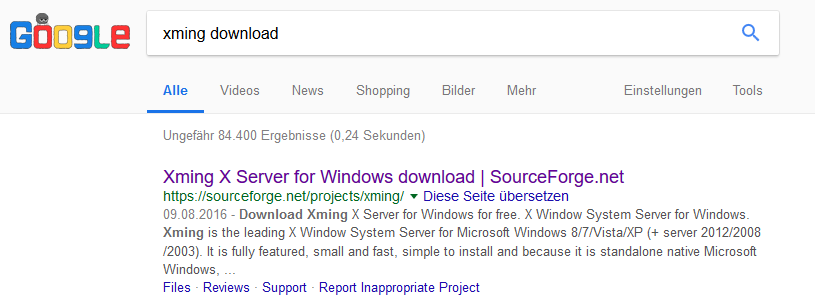
\includegraphics[scale=0.7]{Bilder/Xming.PNG}
\caption{Download Xming}
\label{fig:Xming}
\end{figure}\\ \\Nach dem Download der Installationsanweisung folgen und das Programm Xming starten, nicht den Xming Launcher! Xming läuft nun im Hintergrund und kann jederzeit über die Taskleiste beendet werden.

\subsection{Freischaltung des Features}
Um das Windows Subsystem für Linux zu aktivieren, muss zuerst das Feature aktiviert werden. Dafür öffnet man die Windows PowerShell als Administrator und führt folgenden Befehl aus:
\begin{lstlisting}[language=bash]
Enable-WindowsOptionalFeature -Online -FeatureName Microsoft-Windows-Subsystem-Linux
\end{lstlisting}

Zum Schluss noch mit \textit{Y} bestätigen um den Rechner neu zu starten.

\begin{figure}[H]
\centering
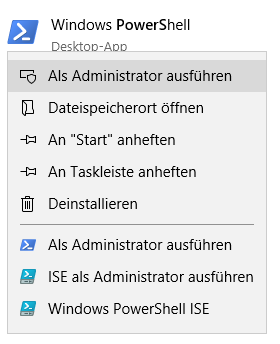
\includegraphics[scale=0.8]{Bilder/PowerShell.PNG}
\caption{Windows PowerShell}
\label{fig:PowerShell}
\end{figure}

\begin{figure}[H]
\centering
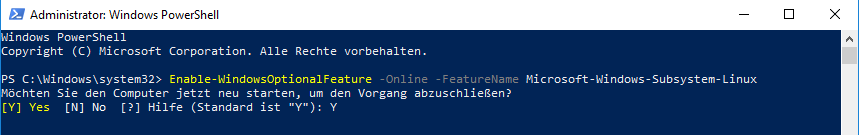
\includegraphics[scale=0.5]{Bilder/Befehl.PNG}
\caption{Befehl}
\label{fig:Befehl}
\end{figure}



\subsection{Installation von Ubuntu}
Die passende Installation von Ubuntu für das Subsystem findet man im Microsoft Store.

\begin{figure}[H]
\centering
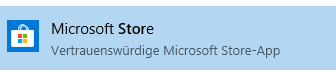
\includegraphics[scale=1]{Bilder/Store.PNG}
\caption{Microsoft Store}
\label{fig:Store}
\end{figure}

Dort sucht man nach Ubuntu und installiert es.

\begin{figure}[H]
\centering
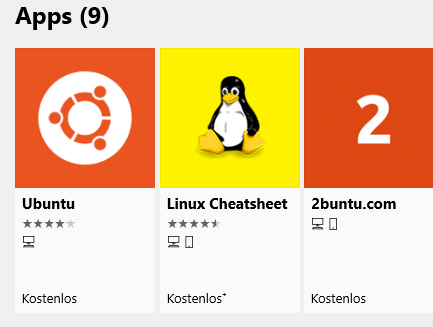
\includegraphics[scale=0.8]{Bilder/Ubuntu.PNG}
\caption{Ubuntu}
\label{fig:Ubuntu}
\end{figure}

\subsection{Einrichten von Ubuntu}
\subsubsection{Anlegen eines Benutzers}
Nach erfolgreicher Installation wird man nun aufgefordert, einen neuen Benutzer anzulegen.

\subsubsection{Testen der grafischen Oberfläche}
Bevor man Xming als X-Server verwenden kann, muss das Display bei jedem Start aktiviert werden. Damit dieser Vorgang bei jedem Start des Subsystems ausgeführt wird, muss folgendes in die Datei \textit{.bashrc} geschrieben werden:\\
Zuerst muss in das Root-Verzeichnis gewechselt werden:
\begin{lstlisting}[language=bash]
cd
\end{lstlisting}

Jetzt kann die Datei mit dem Nano Texteditor geöffnet werden:
\begin{lstlisting}[language=bash]
nano .bashrc
\end{lstlisting}

Folgender Befehl wird jetzt ganz unten eingefügt:
\begin{lstlisting}[language=bash]
export DISPLAY=:0
\end{lstlisting}
Zum Speicher \textit{STRG+O} drücken und zum beenden \textit{STRG+X}.

Danach werden die benötigten Pakete installiert:
\begin{lstlisting}[language=bash]
sudo apt-get install x11-apps
\end{lstlisting}
Jetzt kann die grafische Ausgabe getestet werden:

\begin{lstlisting}[language=bash]
xclock
\end{lstlisting}
Es sollte nun ein Fenster geöffnet werden, auf dem eine Uhr abgebildet ist. Ist dies der Fall, funktioniert der X-Server.
\begin{figure}[H]
\centering
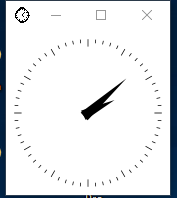
\includegraphics[scale=0.8]{Bilder/Clock.PNG}
\caption{XClock}
\label{fig:XClock}
\end{figure}

\subsubsection{Installation eines grafischen Terminals}
Da für die Verwendung von ROS mehrere Terminals benötigt werden, wird ein grafisches Terminal installiert, das über eine Tabverwaltung verfügt. Mit dem folgendem Befehl lässt sich das Terminal Sakura installieren.
\begin{lstlisting}[language=bash]
sudo apt-get install sakura
\end{lstlisting}
Zum ausführen des Terminals, folgenden Befehl in die Windows Bash eintippen:
\begin{lstlisting}[language=bash]
sakura
\end{lstlisting}
Jetzt öffnet sich in einem seperaten Fenster ein weiteres Terminal das ab sofort das Hauptterminal ist. Nun ist es möglich mit der rechten Maustaste weitere Tabs zu öffnen.



\subsection{Starten von Ubuntu}
Nach der Installation landet man automatisch in der Ubuntu-Umgebung. Möchte man aber nach einem Neustart Ubuntu ausführen, muss folgender Befehl in die Windows Eingabeaufforderung(CMD) eingegeben werden:
\begin{lstlisting}[language=bash]
bash
\end{lstlisting}

\begin{figure}[H]
\centering
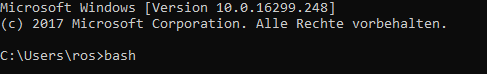
\includegraphics[scale=1.0]{Bilder/Bash.PNG}
\caption{Bash}
\label{fig:Bash}
\end{figure}

\subsection{Beenden von Ubuntu}
Zum beenden von Ubuntu müssen alle grafischen Terminals geschlossen werden, bis auf die Windows Bash. In der Windows Bash kommt man nun mit folgendem Befehl wieder auf das Windows Betriebssystem und beendet damit Ubuntu:
\begin{lstlisting}[language=bash]
exit
\end{lstlisting}
